\documentclass{article}%
\usepackage{lmodern}%
\usepackage{tikz}
\usepackage{calc,graphicx}
\usepackage{graphics}
\usepackage[utf8]{inputenc}
\usepackage[margin=1in,headsep=1cm,headheight= 1in,top=1.5in]{geometry}
\usepackage{fancyhdr}
\usepackage{lastpage}
\usepackage{circuitikz}
\usepackage{multicol}
\usepackage{amsmath}
\usepackage{amssymb}
\usepackage{float}
\usepackage{subcaption}
\usepackage{titlesec,titletoc}
\usepackage{tikz}
\usepackage{lastpage}
\usepackage{pdfpages}
\usepackage[framemethod=tikz]{mdframed}
\usepackage{hyperref}
\usepackage{parskip}
\usepackage{indentfirst}	%para sangrar el primer parrafo luego de una sección
	\hypersetup{
		colorlinks,
			citecolor=black,
			filecolor=black,
			linkcolor=blue,
			urlcolor=red
	}

	\newmdenv[align=center,linewidth=2pt,font=\sffamily,rightmargin=20pt]{caja}

\renewcommand{\contentsname}{Índice}
\renewcommand{\familydefault}{\sfdefault}%
\graphicspath{ {imagenes/} }

\tikzstyle{T1Box} = [fill=teal!20,text width=3cm,inner sep=3.2mm,rounded corners,draw=teal!80,line width=2pt,node distance=4.5cm and 7cm]
\tikzstyle{T1Frecha} = [->,>=stealth,draw=teal!80,line width=3pt]

\title{Proyecto Jefatura de Área}
\date{\today}
\author{Esteban Lemos}

\titleformat{name=\section}[block]
	{\sffamily\bfseries\Large}
	{}
	{0pt}
	{\colorsection}
		\titlespacing*{\section}{0pt}{\baselineskip}{\baselineskip}

		\newcommand{\colorsection}[1]{%
		\colorbox{teal!50}{\parbox{\dimexpr\textwidth-2\fboxsep}{\thesection\ #1}}}

\begin{document}

% membrete ---------------------------------------------------------------------------------------------------------------------------------------------------------------------
	\begin{flushright}
		    PROVINCIA DE BUENOS AIRES\linebreak%
			DIRECCIÓN GENERAL DE CULTURA Y EDUCACIÓN\linebreak%
			DIRECCIÓN DE EDUCACIÓN TÉCNICA\linebreak%
			\textbf{ESCUELA DE EDUCACIÓN SECUNDARIA TÉCNICA Nro. 1}\linebreak%
			\textbf{"EDUARDO ADER"}\linebreak%
			CERRITO 3966 VILLA ADELINA (1607)\linebreak%
			TEL: 47350174
	\end{flushright}
	\begin{tikzpicture}[remember picture,overlay]
		\node [xshift =1in+3.5cm/2, yshift =-(2in)] at (current page.north west){
			
\includegraphics[width=3.5cm]{logo2.jpg}};
	\end{tikzpicture}\vspace{4ex}%

% Carátula ---------------------------------------------------------------------------------------------------------------------------------------------------------------------
	\begin{center}
		
		\fontsize{40}{4}{\textbf{\textcolor{teal}{Proyecto}}}\linebreak \\%
		\vspace{8ex}
		\fontsize{40}{4}{\textbf{\textcolor{teal}{Sistema de Gestión Institucional}}}\linebreak\\%
		\vspace{8ex}		
		\huge{\textbf{Jefatura de Área E.E.S.T. N$^\circ$ 1 Vicente López}}\linebreak\\%
	\end{center}\vspace{2cm}%

	% Colaboradores, actuales directivos

		\begin{large}
			\begin{tabular*}{\linewidth}[]{l l}
				\textbf{Director} : 		&Ezequiel Torres\\
				\textbf{Vicedirector} : 	&Daniel Segnini\\
				\textbf{Vicedirectora} :	&Karin Cuervo\\
				\textbf{Vicedirectora} :	&Mariana Bonetti\\
				\textbf{Secretaria} : 		&Cristina Gómez\\
				\textbf{Jefe de Área} : 	&Esteban Lemos\\
				\textbf{Jefe de Preceptores} : 					&Verónica Victorello\\
				\textbf{Jefe del Dpto. Técnico Profesional} : 	&Alejandro Hsia\\
			\end{tabular*}
		\end{large}\linebreak\\%
		\vspace{1cm}

		\begin{center}
			-- Octubre 2024 --
		\end{center}

		\newpage%

		\tableofcontents{}%
		

\clearpage

%El encabezado----------------------------------------------------------------------------------------------------------------------------------------------------------------

\renewcommand{\footrulewidth}{2pt}
\renewcommand{\headrulewidth}{2pt}
\pagestyle{fancy}
	\rfoot{\thepage\ de \pageref{LastPage}}
	\fancyhead{}
	\cfoot{\footnotesize\textbf{ Escuela de Educación Secundaria Técnica N$^\circ$ 1 - Vicente López}\\Cerrito N$^\circ$ 3966 (1605) Villa Adelina, Partido de Vicente López.\\Tel:(011) 47350174 -- email: tecnica1vl@gmail.com}

	\lhead{\begin{tikzpicture}
		\node (0,0)[]{
\includegraphics[width=0.5in]{logo2.jpg}};
		\node [text width=8cm,align=left,xshift=5cm] at (0,0){\textbf{Proyecto de Gestión Institucional 2024}\linebreak Jefatura de Área\linebreak E.E.S.T. N$^\circ$ 1 V.L.} ;
		\end{tikzpicture}
	}
	\rhead{\rightmark}

%El Documento-----------------------------------------------------------------------------------------------------------------------------------------------------------------
\setlength{\parindent}{1em}



\section{Fundamentación}
	En vista del ACTA-2024-28451026 que indica los procedimientos de intervención con  alumnos que requieren estrategias didácticas y pedagógicas particularizadas.

Tal como se explicita en la Res. CFE 14/07. “La educación técnico profesional introduce a los estudiantes, jóvenes y adultos, en un recorrido de profesionalización a partir del acceso a una base de conocimientos y de habilidades profesionales que les permita su inserción en áreas ocupacionales cuya complejidad exige haber adquirido una formación general, una cultura científico - tecnológica de base a la par de una formación técnica específica de carácter profesional, así como continuar aprendiendo durante toda su vida. Procura, además, responder a las demandas y necesidades del contexto socio productivo en el cual se desarrolla, con una mirada integral y prospectiva que excede a la preparación para el desempeño de puestos de trabajo u oficios específicos”.

Atendiendo a la Res. CFE Nro. 148/11 Anexo I Marco de referencia para procesos de homologación de títulos del nivel secundario Sector Informático, donde se establecen las bases del perfil profesional y que explicitan las competencias del técnico en programación.

Dado que un grupo de alumnos que se encuentran cursando el 5to año de la carrera Técnico en Programación, cuentan con inquietudes particulares y manifiestan gran capacidad de aprendizaje, autonomía y responsabilidad más allá de la esperada para el rango etario.

Que parte de los integrantes de este grupo de alumnos ha participado de proyectos ganadores de feria de ciencias que han sido valorados dentro y fuera de la comunidad de la Técnica 1.

\section{Objetivo}
	Se propone para dicho grupo y con un alcance particular para cada uno de sus integrantes, un proyecto integrador de gran interés para la institución; dicho proyecto será llevado a cabo en el tiempo restante del ciclo lectivo 2024 y tendrá continuidad en los próximos ciclos teniendo en cuenta que los alumnos se encontrarán cursando hasta su egreso en el 2026.

Se busca de esta manera generar la motivación necesaria para que este grupo de alumnos pongan en juego todo su conocimiento y potencial, adquiera las competencias necesarias para la acreditación de los espacios y aporten a la comunidad educativa de la Escuela de Educación Secundaria Técnica Nro. 1, una herramienta de gestión que permita un mejor seguimiento de los aprendizajes de los estudiantes desde su ingreso en 1er año hasta su egreso en 7mo. así como la implementación del nuevo régimen académico en forma orgánica.

\section{Acuerdos}
	En el presente documento se detallan las condiciones para la acreditación de saberes propios de la especialidad de la carrera de Técnico en Programación de materias técnico específicas y de formación científico tecnológica para estudiantes afectados al Proyecto “Sistema de Gestión Institucional de la EEST1”.

Dichas condiciones se especifican para cada uno de los estudiantes en particular a excepción de aquellos donde no se menciona de manera individualizada, en cuyo caso se entiende que aplica a todos y cada uno de ellos. 

Los estudiantes alcanzados por las especificaciones del presente documento, todos pertenecientes al 5to 3ra del ciclo lectivo 2024 de la carrera de programación, son:

    \begin{itemize}
        \item Julián Gonzalez.
        \item Bautista Izaguirre.
    \end{itemize}

\subsection{Materias no incluidas en el proyecto}

Estas materias no están directamente relacionadas con el proyecto “Sistema de Gestión Institucional” de la EEST1,  que los estudiantes están realizando y, por tanto, no se encuentren alcanzados por las condiciones del presente documento. Esto significa que deberán cursarse y acreditarse según los medios habituales incluyendo las condiciones de presentismo y promoción.

\subsubsection{Análisis Matemático. (prof. Olmos )}
\subsubsection{Sistemas Digitales I (prof. Salimbeni)}

\subsection{Materias con acreditación parcial}

Son aquellas que son alcanzadas por el proyecto, pero que dadas sus condiciones de promoción, serán acreditadas parcialmente mediante la entrega del "Sistema de Gestión Institucional", siendo necesario cumplimentar trabajos y/o entregas complementarios/as en la cursada.

A continuación se detallan las condiciones particulares acordadas con y entre los profesores para las materias:

\subsubsection{Base de Datos (prof. Balda)}       

El programa actualizado de la materia se encuentra en el Centro de Recursos Multimediales y se puede consultar ingresando la dirección en la barra del explorador o haciendo clic en el siguiente enlace:

\url{https://drive.google.com/drive/folders/1BbvXoqqAXC5Uq4ZXNdTD-EYfUl_R2YkI?usp=drive_link}.

La profesora hace entrega al equipo Directivo y Jerárquico un documento detallando su plan de trabajo para el desarrollo del proyecto "Sistema de Gestión Institucional". Este documento se adjunta al presente proyecto en el apartado de Anexos.

A modo de resumen se presentan los siguientes aspectos:
\paragraph{Expectativas de Logro}
Se espera que los estudiantes adquieran habilidades y conocimientos que les permitan: 
\begin{itemize}
    \item Crear una base de datos relacional.
    \item Implementar un motor de base de datos.
    \item Gestionar una base de datos.
    \item Comprender y aplicar comandos SQL. 
\end{itemize}


\paragraph{Evaluación y acreditación del docente}
Los estudiantes deberán presentar y exponer el proyecto "Sistema de Gestión Institucional" utilizando el vocabulario específico de la materia y respetando las siguientes condiciones:
\begin{itemize}
    \item Se deberá respetar el formato de la presentación indicado por el docente.
    \item Deberán incluir un informe de los temas indicados en el anexo.
    \item Deberán conocer la bibliografía indicada en el anexo y aplicar los fundamentos allí estudiados
\end{itemize}
\paragraph{Bibliografía} Los alumnos deberán utilizar el material indicado por el docente:
\begin{itemize}
    \item Marqués-Andrés, M. (2011). Bases de datos. Universitat Jaume I.
    \item  Oppel, A., \& Sheldon, R. (2008). SQL. McGraw-Hill Professional Publishing.
\end{itemize}

\subsubsection{Modelos y Sistemas (prof. Insaurralde)}.

El programa actualizado de la materia se encuentra en el Centro de Recursos Multimediales y se puede consultar ingresando la dirección en la barra del explorador o haciendo clic en el siguiente enlace:

\url{https://drive.google.com/drive/folders/1BbvXoqqAXC5Uq4ZXNdTD-EYfUl_R2YkI?usp=drive_link}.

Este espacio se relaciona íntegramente con el proyecto y tanto la dinámica como los objetivos propuestos por el docente se alinean perfectamente con los requerimientos del sistema que los alumnos deben desarrollar. Por eso la acreditación del espacio estará completamente a cargo del docente.

\paragraph{Expectativas de Logro} Finalizada la cursada del espacio los alumnos tendrán conocimientos y capacidades para:

\begin{itemize}
    \item Realizar programación estructurada y secuencial. 
    \item Utilizar herramientas específicas para la diagramación de flujo de datos.
    \item Comprender y realizar ciclos anidados mediante modelos ER y formas normales utilizando PK y FK.
    \item Realizar la documentación necesaria para un sistema informático.
\end{itemize}

\paragraph{Evaluación} Para el visado final, los alumnos deberán entregar al docente:
\begin{itemize}
    \item Manual del Sistema o del Programador.
    \item Manual de Usuario.
\end{itemize}

\paragraph{Bibliografía} Los alumnos tendrán acceso al siguiente material bibliográfico:

\begin{itemize}
    \item Santiago Ramírez (1999). Teoría General de los sistemas de Bertalanffy. Universidad Autónoma de México. Capítulo 3 y 4.
    \item Bonatti(2011). Teoría de la decisión. Editorial Prearson.
    \item Pablo Sznajdleder(2012). Algoritmos a fondo con implementaciones en c y java. Editorial Alfaomega.
\end{itemize}


\subsection{Materias con acreditación conjunta}

Son aquellas que son alcanzadas en su totalidad por el proyecto, las mismas se acreditan mediante la presentación del "Sistema de Gestión Institucional" cumpliendo con la totalidad de los objetivos propuestos.

\paragraph{Evaluación y acreditación} El equipo directivo y los docentes se reunen en comisión al finalizar el segundo cuatrimestre para analizar la funcionalidad del sistema. Durante el período de intensificación de diciembre se realizan pruebas de funcionamiento, siendo depurado el código del sistema hasta no presentar errores de gravedad o críticos. Al finalizar el ciclo lectivo los modulos solicitados en la inclusión del sistema deberán ser completamente funcionales.



\subsubsection{Laboratorio de Diseño de Bases de Datos (prof. Sanfelice - prof. Ganduglia)} 

El programa actualizado de la materia se encuentra en el Centro de Recursos Multimediales y se puede consultar ingresando la dirección en la barra del explorador o haciendo clic en el siguiente enlace:

\url{https://drive.google.com/drive/folders/1BbvXoqqAXC5Uq4ZXNdTD-EYfUl_R2YkI?usp=drive_link}.

Los profesores entregan al equipo Directivo y Jerárquico un plan de trabajo basado en proyectos. Este plan divide en grupos al total de los alumnos que cursan la materia y a cada grupo se le asigna una problemática diferente a resolver. El proyecto "Sistema de Gestión Institucional" es totalmente compatible con la modalidad de trabajo planteada por los docentes.

A modo resumen se presentan los siguientes aspectos:
\paragraph{Expectativas de Logro}
Se espera que los estudiantes adquieran habilidades y conocimientos que les permitan: 

\begin{itemize}
    \item Crear de bases de datos.
    \item Comprender y aplicar el modelo relacional.
    \item Mantener y gestionar bases de datos propias o de terceros.
    \item Crear módulos e interfaces para el acceso seguro de usuarios.
    \item Interpretar y crear consultas mediante lenguaje SQL.
    \item Implementar y mantener servidores y motores de bases de datos. 
\end{itemize}

\paragraph{Evaluación y acreditación}

Los estudiantes deberán presentar y exponer el proyecto "Sistema de Gestión Institucional" depurado y sin errores críticos, o que revistan gravedad, en su funcionamiento. Los docentes de los espacios incluidos en los apartados 3.2 y 3.3, especialistas del área, analizan en conjunto con el equipo Directivo y Jerarquico los aspectos técnicos y la correcta implementación del sistema así como también la utilización de las buenas prácticas de programación.

\paragraph{Bibliografía} Los docentes recomiendan a los estudiantes el siguiente material de consulta:

\begin{itemize}
    \item Aguirre Juan, (2009). Bases de datos en MySQL 
    \item Sánchez, J. (2004). Principios sobre bases de datos relacionales. Informe, Creative Commons, 11, 20.
    \item Minera, F. (2011). Desarrollo PHP y MySQL. USERSHOP.
\end{itemize}
   %Laboratorio de base de datos.
\subsubsection{Laboratorio de Programación (prof. Sanfelice - prof. Ganduglia)}

El programa actualizado de la materia se encuentra en el centro de recursos multimedia y puede ser accedido ingresando la dirección en la barra del explorador o haciendo click en el link :


\url{https://drive.google.com/drive/folders/1BbvXoqqAXC5Uq4ZXNdTD-EYfUl_R2YkI?usp=drive_link}



Los profesores entregan al equipo Directivo y Jerárquico un plan de trabajo basado en proyectos, donde el total de los alumnos que cursan la materia se dividen en grupos, a los mismos se les asignan diferentes proyectos y situaciones problemáticas a resolver, por lo cual el "Sistema de Gestión Institucional", es totalmente compatible con la modalidad de trabajo planteada por los docentes.

A modo resumen se presentan los siguientes aspectos:
\paragraph{Espectativas de Logro}
Se espera que los estudiantes adquieran habilidades y conocimientos que les permitan: 

\begin{itemize}
    \item Utilizar lenguajes de programación estructurados.
    \item Utilizar lenguajes de programación orientados a objetos.
    \item Resolver problemas sencillos mediante la creación de programas / algoritmos.
    \item Mantener, Revisar y depurar software.
    \item Utilizar herramientas para el control de versiones.
    \item Desarrollar soluciones de gestión a nivel macro aplicando todas las herramientas de desarrollo actuales. 
\end{itemize}

\paragraph{Evaluación y acreditación}

Los estudiantes deberán presentar y exponer el Proyecto Integrador Final "Sistema de Gestión Institucional", depurado y sin errores graves o críticos en el funcionamiento del mismo. Los docentes especialista del área analizan en conjunto con el equipo directivo y Jerarquico los aspectos técnicos y la correcta implementación, así como el uso de buenas prácticas de programación.

\paragraph{Bibliografía}
\begin{itemize}
    \item  (Luis Joyanes Aguilar, Ignacio Zahonero Martínez). Programación en C, C++, Java y UML - McGRAW-HILL Education

\end{itemize}     %Laboratorio de Programación.
\subsubsection{Laboratorio de Diseño Web (prof. González - prof. Ganduglia)}
El programa actualizado de la materia se encuentra en el Centro de Recursos Multimediales y se puede consultar ingresando la dirección en la barra del explorador o haciendo clic en el siguiente enlace:

\url{https://drive.google.com/drive/folders/1BbvXoqqAXC5Uq4ZXNdTD-EYfUl_R2YkI?usp=drive_link}.

Los profesores entregan al equipo Directivo y Jerárquico un plan de trabajo basado en proyectos, donde el total de los alumnos que cursan la materia se dividen en grupos, a los mismo se les asignan diferentes proyectos a resolver, por lo cual el "Sistema de Gestión Institucional", es totalmente compatible con la modalidad de trabajo planteada por los docentes.

A modo resumen se presentan los siguientes aspectos:
\paragraph{Expectativas de Logro}
Se espera que los estudiantes adquieran habilidades y conocimientos que les permitan: 

\begin{itemize}
    \item Creación de páginas web mediante el uso del HTML.
    \item Creación de estilos mediante el uso de CSS.
    \item Publicación de páginas y uso de servidores APACHE.
    \item Creación de formularios e integración con bases de datos.
    \item Realización de consultas mediante el uso de lenguaje PHP.

\end{itemize}

\paragraph{Evaluación y acreditación}

Los estudiantes deberán presentar y exponer el Proyecto Integrador Final "Sistema de Gestión Institucional", depurado y sin errores graves o críticos en el funcionamiento del mismo. Los docentes especialista del área analizan en conjunto con el equipo directivo y Jerarquico los aspectos técnicos y la correcta implementación así como el uso de buenas prácticas de programación.

\paragraph{Bibliografía} Los docentes recomiendan a los estudiantes el siguiente material de consulta:

\begin{itemize}
    \item Beati, H. (2020). HTML5 y CSS3 para diseñadores. Marcombo.
\end{itemize}
    %Laboratorio de Diseño Web.
\subsubsection{Laboratorio de Redes Informáticas (prof. Sanfelice - prof. Figueroa)}.

El programa actualizado de la materia se encuentra en el Centro de Recursos Multimediales y se puede consultar ingresando la dirección en la barra del explorador o haciendo clic en el siguiente enlace:

\url{https://drive.google.com/drive/folders/1BbvXoqqAXC5Uq4ZXNdTD-EYfUl_R2YkI?usp=drive_link}

Los profesores entregan al equipo Directivo y Jerárquico un plan de trabajo basado en proyectos. Este plan divide en grupos al total de los alumnos que cursan la materia y a cada grupo se le asigna una problemática diferente a resolver. El proyecto "Sistema de Gestión Institucional" es totalmente compatible con la modalidad de trabajo planteada por los docentes.

A modo de resumen se presentan los siguientes aspectos:
\paragraph{Expectativas de Logro}
Se espera que los estudiantes adquieran habilidades y conocimientos que les permitan: 

\begin{itemize}
    \item item
\end{itemize}

\paragraph{Evaluación y acreditación}

Los estudiantes deberán presentar y exponer el proyecto "Sistema de Gestión Institucional" depurado y sin errores críticos, o que revistan gravedad, en su funcionamiento. Los docentes de los espacios incluidos en los apartados 3.2 y 3.3, especialistas del área, analizan en conjunto con el equipo Directivo y Jerarquico los aspectos técnicos y la correcta implementación del sistema así como también la utilización de las buenas prácticas de programación.

\paragraph{Bibliografía} Los docentes recomiendan a los estudiantes el siguiente material de consulta:
\begin{itemize}
    \item  

\end{itemize}
    %Laboratorio de redes informáticas


\section{Enunciado}
	Los estudiantes involucrados en el presente proyecto estarán encargados de desarrollar un "Sistema de Gestión Institucional". Se prevé un plazo de tres años para su finalización. La extensión del proyecto incluye el 5to, 6to y 7mo año de los estudiantes interesados.

En esta primera etapa de desarrollo deberán entregar un sistema parcial formado por los siguientes módulos:

\begin{itemize}
    \item Módulo Pañol.
    \item Módulo de Inscripción.
    \item Módulo de Asistencia.
    \item Módulo ABM de alumnos y profesores
\end{itemize}

Cada módulo tendrá una fecha de entraga previamente establecida. El plazo de entrega final para este sistema parcial será hasta la finalización del ciclo lectivo 2024.

Los módulos deben ser accesibles a través de un portal WEB alojado en el servidor de la institución. Solo podrán acceder usuarios que se encuentren dentro de la intranet.

\subsection{Módulo Pañol}

Diariamente en la escuela, los alumnos que cursan materias con modalidad de taller solicitan herramientas e instrumental para avanzar con los proyectos y actividades propuestas. Si bien las herramientas se encuentran a cuidado de los EMATP pañol, se hace evidente la necesidad de herramientas de gestión de inventario a la hora de mejorar las tareas asociadas al prestamo de los elementos siendo los puntos a mejorar:

\begin{itemize}
    \item Búsqueda rápida de herramientas. Dado que la ubicación y cantidad disponibles están al alcance de todos los usuarios del sistema.
    \item Control de inventario.
    \item Mejora de los tiempos de altas y bajas de herramientas e instrumental.
    \item Mejora de los tiempos de solicitud de herramientas e instrumental.
    \item Mejora de los tiempos de entrega y devolución de herramientas e instrumental
\end{itemize}
\subsubsection{Módulo Pañol (solicitud)}
Se solicita a los estudiantes un módulo que permita a traves de los dispositivos móviles con los que cuentan los estudiantes y profesores, realizar búsquedas de herramientas y solicitar y/o reservar los elementos del inventario.
\subsubsection{Módulo Pañol (entrega)}
Se solicita a los estudiantes un módulo que permita al EMATP pañol a partir de una computadora instalada en dicho pañol o un dispositivo movil, recibir solicitudes y realizar las entregas de los elementos requeridos.
\subsubsection{Módulo Pañol (devolución)}
Se solicita a los estudiantes un módulo que permita a los docentes y al EMATP pañol a partir de una computadora instalada en dicho pañol o un dispositivo movil, registrar las devoluciones de los elementos prestados.

\subsubsection{Módulo Pañol (invetario)}
Se solicita a los estudiantes un módulo que permita al EMATP pañol realizar controles periódicos del estado del inventario pudiendo asentar informes de la situación.


\subsection{Módulo de Inscripción}

Los aspirantes a vacantes para el primer año realizan una preinscripción durante el mes de diciembre. Este módulo debe permitir a las familias realizar esta preinscripción a través de terminales instaladas en la escuela. La inscripción efectiva se completará con la incorporación de la documentación respaldatoria que conformará el lejago digital.

Este módulo debe encontrarse operativo antes de este período.

\subsection{Módulo de Asistencia}

Este módulo permite tomar asistencia a los alumnos que se encuentren inscriptos en las distintas materias dentro de sus correspondientes años. La implementación de este módulo está prevista para el ciclo lectivo 2025.

Este módulo debe encontrarse operativo antes de dar inicio al ciclo lectivo 2025.

Este registro debe contemplar la generación de informes que den cuenta de las distintas ponderaciones de asistencia.

\subsection{Módulo ABM}

Este módulo deberá contener todos los cámpos necesarios para poder agregar, modificar, corregir y respaldar toda la información que se encuentra contenida en los legajos de los alumnos y los docentes.

En una primera instancia, el grupo de desarrollo deberá coordinar con el equipo Directivo y Jerárquico la carga de datos de todos los alumnos y verificar que todos cuentan con perfiles de usuario. Estos perfiles no deben tener permisos para ingresar ni editar ningún dato.
	
\section{Evaluación Colegiada}
Al finalizar la cursada regular, los estudiantes deberán hacer una presentación del trabajo realizado donde expondrán el funcionamiento del "Sistema de Gestión Institucional" frente al equipo Directivo, el Jefe de Área y los docentes de los espacios consignados en los apartados 3.2 y 3.3. Esta presentación deberá incluir:

\begin{itemize}
    \item El Manual de Usuario impreso.
    \item El Manual del Programador impreso.
    \item Una presentación multimedia.
    \item Una lista de tutoriales. 
\end{itemize}

\subsection{Manual de Usuario}

El Manual de Usuario será un requisito para la acreditación del espacio \textbf{Modelos y Sistemas}. Este deberá contener de manera  sistemática y ordenada la guía para el uso de todas las funciones de cada módulo del sistema organizadas por perfil.

\subsection{Manual del Programador}

El Manual del Programador será un requisito para la acreditación del espacio \textbf{Modelos y Sistemas}. Este deberá contener de manera sistemática y ordenada la documentación requerida para el mantenimiento de cada módulo del sistema así como también toda la información necesaria para la incorporación de nuevos módulos o funciones adicionales.

\subsection{Presentación multimedia}

La presentación debe proporcionar una explicación pormenorizada del funcionamiento de todo el sistema en la cual se ponga de mnifiesto el conocimiento técnico formal aplcado así como también el uso de vocabulario específico. 

\subsection{Lista de tutoriales}

La lista de tutoriales consistirá de una colección de videos organizados por tipo de operación y perfil. Estos serán utilizados para la capacitación del equipo Jerárquico y del cuerpo de preceptores ya que serán los primeros usuarios que tendrá el sistema. 



\newpage	

\section{Anexos}

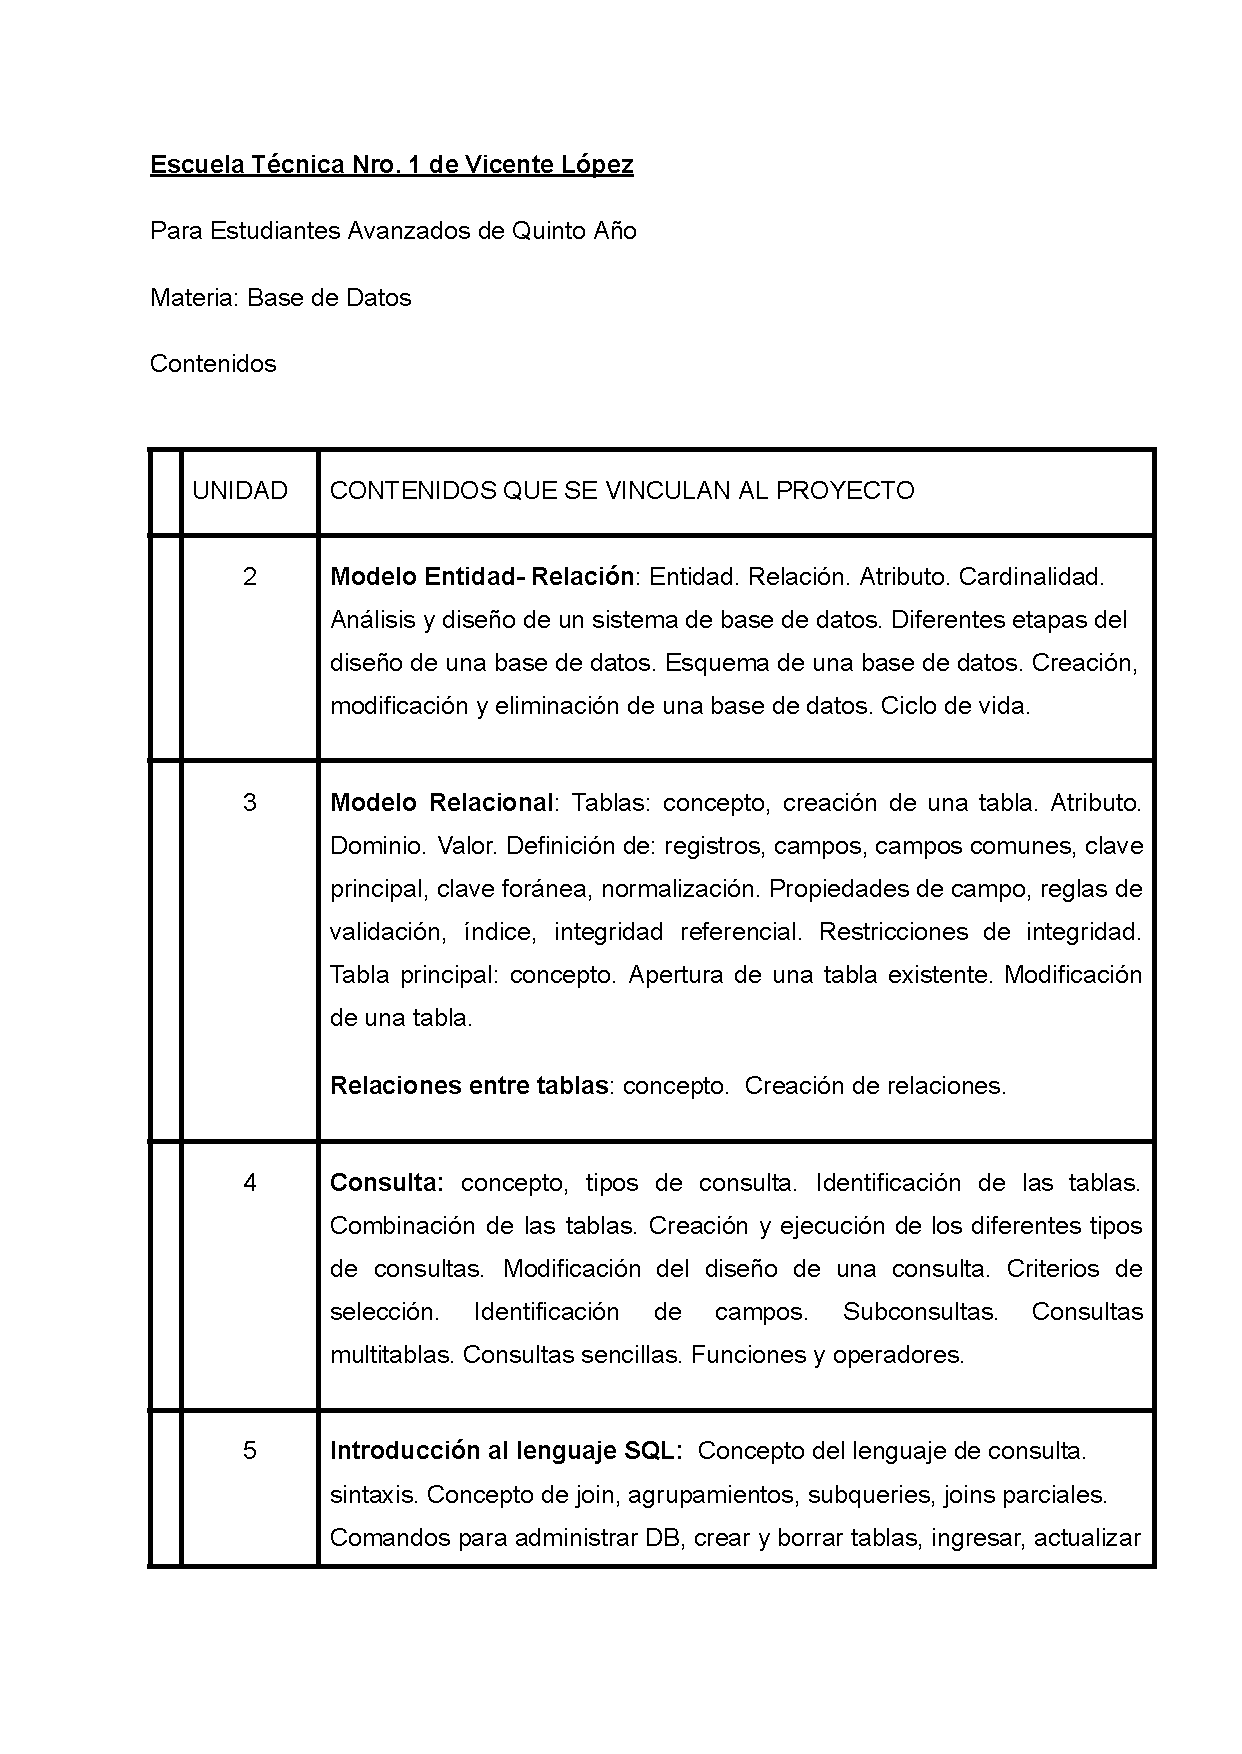
\includepdf[pages=-]{ProyectoBalda.pdf}	
	
\end{document}

